%\begin{figure*}[t!]
\section{Design}
\iffalse
This section describes the design and implementation of \ours{} buffer in detail. 
\S~\ref{subsec:overview} overviews the overall architecture of the in-storage buffer under capacitance constraints, and \S~\ref{subsec:lind_sched} presents the I/O scheduling algorithm
to reduce the write traffic in \ours{}.

\subsection{Overview}
\label{subsec:overview}
To satisfy a high demand for storage capacity in modern applications,
the SSDs have become highly scalable with advances in density-increasing techniques. 
The state-of-the-art SSDs provide tens of TBs capacity and this trend is expected 
to continue in the future.
The problem is that the capacitors, an integral component used in SSDs to protect the buffer data
in power outage, is unable to keep up with the significant density increase speed of NAND flash memory. 
The SSD-internal buffer is typically 0.1\% of the storage capacity in size.
To protect the entire buffer of SSD, the capacitors 
should have been improved at the same pace with SSD in density; 
its density has enhanced only at one-fifth speed of SSD density improvement. 
% This density gap between capacitors and memory technologies
% indicates that 
With this density gap, the PLP with full protection is no longer feasible in SSDs; 
it not only severely limits the form factor of SSDs requiring deployment of a large number of capacitors but also significantly increases the manufacturing cost of SSDs. 

\ours{} is designed to efficiently maintain the in-storage buffer under capacitance limitations. 
Table~\ref{tab:ssd_buff_comp} shows the breakdown of the in-storage buffer usage for each component
for 512GB SSD that has an architecture shown in Table~\ref{tab:ssd_config}. 
The user data buffer is employed to fully exploit the underlying flash parallelism.
Hence, it is typically twice the size of all pages that can be programmed in parallel, 
which is 4MB in this setting, while it may vary depending on the design choice. 
The mapping table that translates LPN(logical page number) to PPN(physical page number) 
accounts for 512MB, which corresponds to 97\% of the buffer size. 
Other metadata including mapping table directory uses a total of 10.5MB buffer. 

To overcome capacitance constraints for SSD, \ours{} sacrifices on some durability of mapping table, 
% by only protecting a portion of it, 
while protecting the user data and the metadata other than mapping table with capacitors. 
The user data persistence should be synchronously guaranteed with the host request
to conserve the properties of existing SSDs with PLP. 
For this reason, making a compromise on it can lead to a serious performance penalty in SSD.
On contrary, the requirements for the mapping table update are less stringent;
it does not have to be immediate upon a host request because the address translation is 
necessary only when the associated data is actually programmed to the flash memory. 
This nature allows a room for reasonable trade-off between capacitance and performance,
by effectively maintaining the persisting overhead of mapping table under capacitance constraint. 
Other metadata updates are also asynchronous with the host request, but
they use only a marginal space of the buffer; sophisticating their management mechanism 
for further capacitance saving is cost-ineffective. 

% because the PPN of data is determined when it is flushed to the flash memory. 
% The LPB to PPN translation is required when the data is in flash memory. 
% it can be restored on the reboot. 

% 요청된 데이터를 찾기 위해 사용. 
% 데이터는 보호되고 있는데 인덱스는 잃어버림. 
% ==> 추후 recovery 할 때 반영해주면 됨. 데이터를 쓰면서 업데이트 하거나 '
% ==> 이미 데이터가 플래시에 쓰여져 있다면? 걔는 보호를 해줘야 함. 
% ==> 대신 small write 임. 버퍼링 효과를 늘리면 footprint 를 줄일 수 있음. 

\iffalse
If an SSD has 8 channels and 4 ways per channel with 8KB page size, about 128KB of memory (twicethe  size  of  all  pages  that  can  be  written  in  parallel)  are  usedfor data buffering. This, however, only accounts for 0.02% ofthe volatile DRAM.
maximize the high degree of parallism in SSDs 
during the operation of flash memories 
\fi

% the end of full protection based SSD design 
%The capacitance faces scaling limit 

% mapping table 이 상당히 큰 부분을 차지한다. 
% 사용자 버퍼는 통상 SSD의 병렬성을 활용할 수 있는 정도로만 있으면 된다고 했지만, 
% 최근 다양한 이유로 증가하고 있음. 

\subsection{Least Increase of Dirtiness Scheduling}
\label{subsec:lind_sched}
\fi
\ours{} partially protects the mapping table with limited capacitance. 
When the dirty pages of mapping table become more than the maximum number of protected pages, 
\ours{} flushes them to flash memory based on the LRU (Least-recently Used) algorithm. 
Because this flush operation does not arise with SSD using PLP, mitigating the effect of this overhead 
is a key strategy to achieving high performance under capacitance constraints. 
To this end, \ours{} presents a cost-effective scheduling scheme for the in-storage buffer.
\ours{} prefers to force the user data that increases the dirtiness of the mapping 
table the least to flash memory. This scheme reduces the dirty page footprint 
of the mapping table at a time window by enhancing the locality of updates. 
As a result, the frequency of flush operation for the mapping table can be 
largely reduced. 

\begin{figure}
    \centering{}
    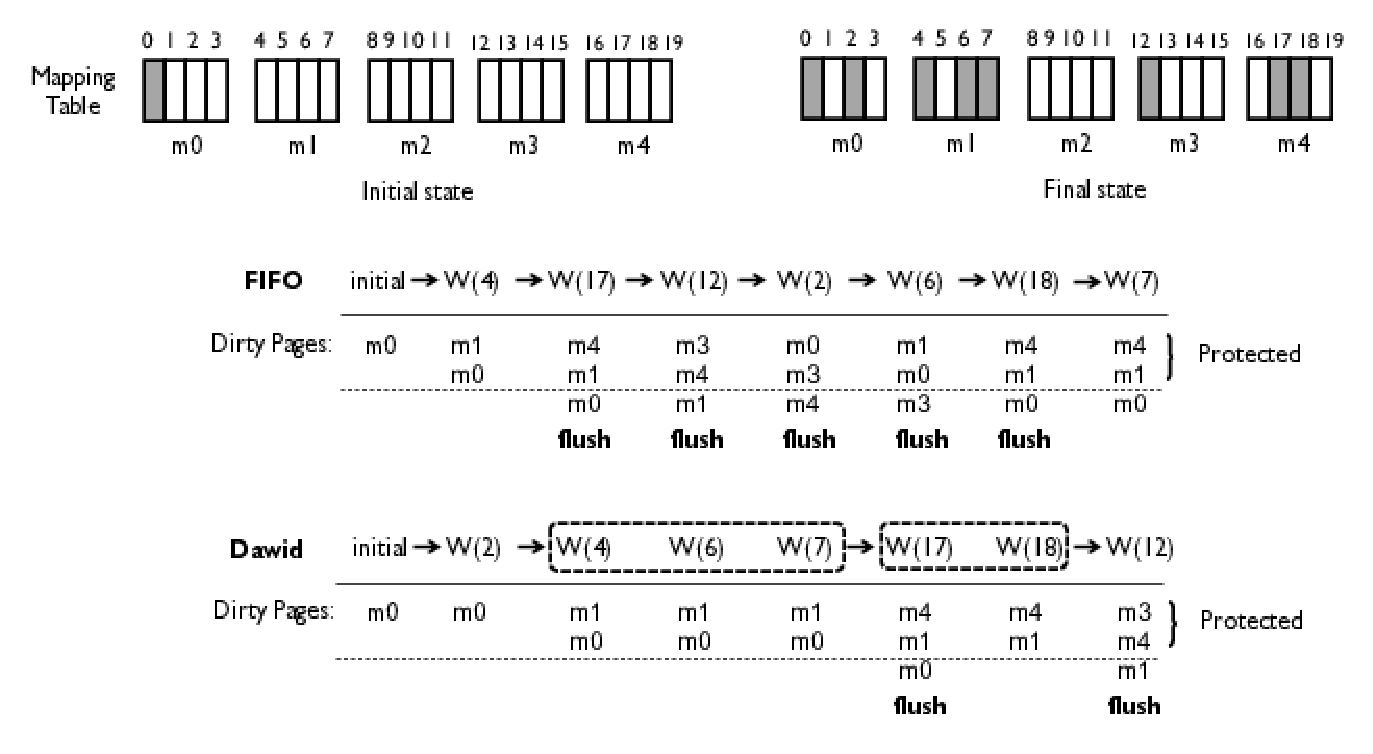
\includegraphics[width=0.5\textwidth]{figure/dawid_algo.eps}
    \caption{\textbf{\ours{}-SSD buffer management scheme}}
    \label{fig:dawid_buff_overview}
\end{figure}


Figure~\ref{fig:dawid_buff_overview} compares the flush overhead of \texttt{FIFO} and \ours{} scheduling in SSD buffer. 
In this example, there are seven write requests 
in the device queue, sent from host in the following order: \texttt{W(4)}, \texttt{W(17)}, \texttt{W(12)}, \texttt{W(2)}, \texttt{W(6)}, \texttt{W(18)}, and \texttt{W(7)}.  
The mapping table has one dirty page (\texttt{m0}) 
at an initial state. We assume that 2 out of 5 pages of the mapping table are protected. 
FIFO writes the user data in the buffer to flash memory in arrival order. 
With this scheme, the mapping table would be randomly updated, generating a large number of dirty pages at a 
time window. 
Consequently, FIFO incurs a total of five flushes of the mapping table page during the write process. 


In contrast, \ours{} calculates the write cost for each data that indicates an
increase in the number of dirty pages of the mapping table when it is flushed,
and it processes the request with minimum cost first.  In this example, the
write request \texttt{W(2)} has a top priority because its associated mapping
table page (\texttt{m0}) is already dirty, and thus it does not add the dirty
pages of the mapping table.  Next, the write requests \texttt{W(4)},
\texttt{W(6)}, and \texttt{W(7)} are processed.  Because their address mapping
entries are located in the same page of the mapping table, the cost of flushing
them is reduced to one third.  With this scheme, \ours{} can reduce the footprint
of mapping table updates within time intervals, thereby delivering only two
flushes of the mapping table for the same task. 

\iffalse
\subsection{Eviction Policy}
\begin{figure}[t!]
    \centering{}
	\subfloat[JESD] { 
    	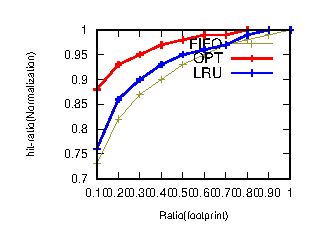
\includegraphics[width=0.2\textwidth]{expr/hitMap/eps/JESD_FIFO.eps}
    	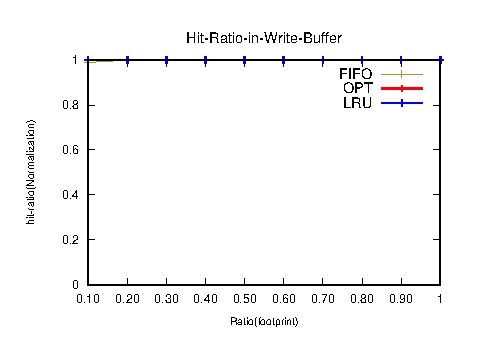
\includegraphics[width=0.2\textwidth]{expr/hitMap/eps/JESD_DAWID.eps}
	} \\
	\subfloat[OLTP]{ 
    	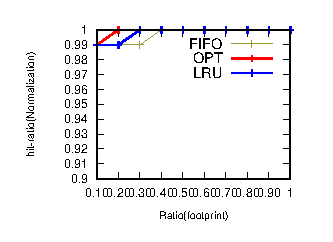
\includegraphics[width=0.2\textwidth]{expr/hitMap/eps/OLTP_FIFO.eps}
    	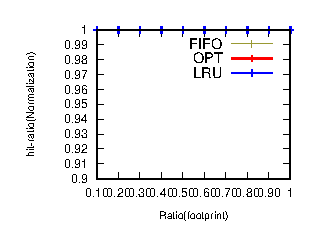
\includegraphics[width=0.2\textwidth]{expr/hitMap/eps/OLTP_DAWID.eps}
	} \\
	\subfloat[Linkbench]{ 
    	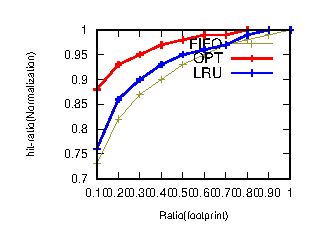
\includegraphics[width=0.2\textwidth]{expr/hitMap/eps/JESD_FIFO.eps}
    	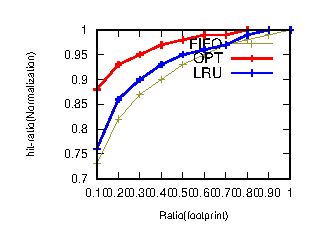
\includegraphics[width=0.2\textwidth]{expr/hitMap/eps/JESD_FIFO.eps}
	} \\
    \caption{\textbf{Write hit ratio for the protected range in a mapping table.}}
    \label{fig_dawid_archi}
\end{figure}
\fi

